\def\made{0103}
\begin{name}
	{Biên soạn \& Phản biện: Nhóm 3}
	{Đề thi chính thức}
\end{name}
\Opensolutionfile{ansbook}[ans/ansb\currfilebase]
\caulc
\Opensolutionfile{ans}[ans/ans\currfilebase-Phan-I]
\begin{ex}%[Dự án 4SJ86V-VN-MT-15+]%[2-TN-0103-BGD-2026,TV035]%[ID6]
	Nghiệm của phương trình $\log_3 (x-1)=1$ là 
	\choice
		{$x=5$}
		{$x=3$}
		{$x=2$}
		{\True $x=4$}
	\loigiai{
		Ta có 
		\[\log_3 (x-1)=1 \Leftrightarrow x-1 =3 \Leftrightarrow x=4.\]
		Vậy phương trình đã cho có nghiệm duy nhất là $x=4$. 
	}
\end{ex}

\begin{ex}%[Dự án FXOM72-VN-MT-15+]%[2-TN-0103-BGD-2026,TV035]%[ID6]
	\immini[thm]{Cho hình lập phương $ABCD.A'B'C'D'$ (xem hình bên). Vectơ nào dưới đây bằng vectơ $\overrightarrow{AB}$?
		\choice[2]
			{$\overrightarrow{CD}$}
			{\True $\overrightarrow{D'C'}$}
			{$\overrightarrow{AA'}$}
			{$\overrightarrow{AD}$}}
			{\begin{tikzpicture}[font=\footnotesize, line join=round, line cap=round, >=stealth,scale=0.8]
    %hidden: VM005
				\foreach \x/\y/\pos in {0/0/A, 3/0/B, -1/-1.2/D} \path ($(\x,\y)$) coordinate (\pos) ($(\x,\y)+(0,3)$) coordinate (\pos'); 
				\path ($(B)+(D)-(A)$) coordinate (C) ($(C)+(0,3)$) coordinate (C'); 
				\draw (A') -- (D') -- (D) -- (C) -- (B) -- (B') -- (C') -- (D') (A') -- (B') (C) -- (C');
				\draw[dashed] (A') -- (A) -- (B) (A) -- (D);
				\foreach \x/\pos in {A/165,B/0,C/-30,D/-150,A'/150,B'/30,C'/-15,D'/180} \fill (\x) circle(1pt) node[{shift=(\pos:0.25)}]{$\x$}; 
    \node at (0,0){\href{FXOM72}{\tiny \phantom{FXOM72}}};
			\end{tikzpicture}}
	\loigiai{
		Vì $ABCD.A'B'C'D'$ là hình lập phương nên ta có $\overrightarrow{AB} = \overrightarrow{D'C'}$.
	}
\end{ex}

\begin{ex}%[Dự án 59HMT8-VN-MT-15+]%[2-TN-0103-BGD-2026,TV035]%[1D6N4-2]
	Cho hai biến cố độc lập $A$ và $B$ có xác suất thỏa mãn $\mathrm{P} (A) =0{,}5$ và $\mathrm{P}(B)=0{,}4$. Giá trị của $\mathrm{P}(AB)$ bằng
	\choice
		{$0{,}9$}
		{$0{,}1$}
		{\True $0{,}2$}
		{$0{,}8$}
	\loigiai{
		Do $A$ và $B$ là hai biến cố độc lập nên 
		\[\mathrm{P}(AB)= \mathrm{P}(A) \cdot \mathrm{P}(B) =0{,}5 \cdot 0{,}4=0{,}2.\]
	}
\end{ex}

\begin{ex}%[Dự án 3B0UAP-VN-MT-15+]%[2-TN-0103-BGD-2026,TV035]%[2D1N4-1]
	Cho hàm số $y=\dfrac{ax+b}{cx+d}$ ($c \ne 0$, $ad-bc \ne 0$) có bảng biến thiên như hình dưới đây: 
	\begin{center}
		\begin{tikzpicture}
    %hidden: VM005
			\tkzTabInit[nocadre=true, lgt=1, espcl=4, deltacl=0.5]
			{$x$/0.7,$y’$/0.7,$y$/2}{$-\infty$,$1$,$+\infty$}
			\tkzTabLine{,+,d,+,}
			\tkzTabVar{-/$-2$,+D-/$+\infty$/$-\infty$,+/$-2$}
    \node at (T11){\href{3B0UAP}{\tiny \phantom{3B0UAP}}};
		\end{tikzpicture}
	\end{center}
	Đường tiệm cận ngang của đồ thị hàm số đã cho có phương trình là 
	\choice
		{$x=-2$}
		{$y=1$}
		{\True $y=-2$}
		{$x=1$}
	\loigiai{
		Dựa vào bảng biến thiên, ta thấy $\lim\limits_{x \to +\infty} y = -2$ và $\lim\limits_{x \to -\infty} y = -2$. \\
		Suy ra đồ thị hàm số $y=\dfrac{ax+b}{cx+d}$ có một đường tiệm cận ngang là $y=-2$.
	}
\end{ex}

\begin{ex}%[Dự án 4HF042-VN-MT-15+]%[2-TN-0103-BGD-2026,TV035]%[2D4H1-3]]
	Cho $\displaystyle\int f(x) \mathrm{\,d}x = \sin x +C$. Phát biểu nào sau đây là đúng? 
	\choice
		{$\displaystyle\int \big[3 +f(x)\big] \mathrm{d}x=3x + \cos x +C$}
		{\True $\displaystyle\int \big[3 +f(x)\big] \mathrm{d}x=3x + \sin x +C$}
		{$\displaystyle\int \big[3 +f(x)\big] \mathrm{d}x=3x - \cos x +C$}
		{$\displaystyle\int \big[3 +f(x)\big] \mathrm{d}x=3x - \sin x +C$}
	\loigiai{
		Ta có 
		\[\displaystyle\int \big[3 +f(x)\big] \mathrm{d}x = \int 3 \mathrm{\,d}x + \int f(x) \mathrm{\,d}x = 3x + \sin x +C.\]
	}
\end{ex}

\begin{ex}%[Dự án 4CS64U-VN-MT-15+]%[2-TN-0103-BGD-2026,TV035]%[1D5N2-2]
	Khảo sát thời gian học trực tuyến (đơn vị: phút) trong một ngày của $42$ học sinh, người ta thu được mẫu số liệu ghép nhóm sau: 
	\begin{center}
		\begin{tabular}{| l | c | c | c | c | c | c |}
			\hline
			Thời gian học trực tuyến &$[10; 20)$&$[20; 30)$&$[30; 40)$&$[40; 50)$&$[50; 60)$&$[60; 70)$ \\ 
			\hline
			Số học sinh &$4$&$8$&$14$&$7$&$4$&$5$\\ 
			\hline
		\end{tabular}
	\end{center}
	Trung vị của mẫu số liệu trên thuộc nhóm nào sau đây? 
	\choice
		{$[50; 60)$}
		{$[60; 70)$}
		{\True $[30; 40)$}
		{$[40; 50)$}
	\loigiai{
		Gọi $x_1$, $x_2$, ..., $x_{42}$ theo thứ tự không giảm là thời gian học trực tuyến của $42$ học sinh. \\
		Vì $x_{21}$, $x_{22} \in [30; 40)$ nên trung vị $M_{\mathrm{e}} = \dfrac{x_{21} + x_{22}}{2} \in [30; 40)$. 
	}
\end{ex}

\begin{ex}%[Dự án 4GI2I1-VN-MT-15+]%[2-TN-0103-BGD-2026,TV013]%[1D2N2-3]
	Cho cấp số cộng $(u_n)$ có $u_1=5$ và công sai $d=-1$. Giá trị của $u_2$ bằng
	\choice
		{$5$}
		{\True $4$}
		{$-4$}
		{$-5$}
	\loigiai{
		Theo công thức số hạng tổng quát của cấp số cộng, ta có
		\[u_2 = u_1 + d = 5 + (-1) = 4.\]
	}
\end{ex}

\begin{ex}%[Dự án 41GY59-VN-MT-15+]%[2-TN-0103-BGD-2026,TV013]%[1D7N2-1]
	Cho các hàm số $y=f(x)$ và $y=g(x)$ có đạo hàm trên tập số thực $\mathbb{R}$ thỏa mãn $f'(x)=x$ và $g'(x)=x^2$. Đạo hàm của hàm số $y=f(x)+g(x)$ là
	\choice
		{\True $x+x^2$}
		{$1+2x$}
		{$1+x^2$}
		{$3x$}
	\loigiai{
		Áp dụng quy tắc đạo hàm của một tổng, ta có
		\[y' = \big[f(x) + g(x)\big]' = f'(x) + g'(x) = x + x^2.\]
	}
\end{ex}

\begin{ex}%[Dự án 2JYO5O-VN-MT-15+]%[2-TN-0103-BGD-2026,TV013]%[2H2N2-3]
	Trong không gian với hệ tọa độ $Oxyz$, cho hai điểm $A(1;5;1)$ và $B(3;3;1)$. Vectơ $\overrightarrow{AB}$ có tọa độ là
	\choice
		{$(4;8;2)$}
		{$(2;4;1)$}
		{\True $(2;-2;0)$}
		{$(-2;2;0)$}
	\loigiai{
		Ta có 
		\[\overrightarrow{AB} = (x_B - x_A; y_B - y_A; z_B - z_A) = (3 - 1; 3 - 5; 1 - 1) = (2; -2; 0).\]
		Suy ra tọa độ của vectơ $\overrightarrow{AB}$ là $(2; -2; 0)$.
	}
\end{ex}

\begin{ex}%[Dự án 2T6M7H-VN-MT-15+]%[2-TN-0103-BGD-2026,TV013]%[0D2N2-1]
	Cặp số nào sau đây là nghiệm của hệ bất phương trình $\heva{&x+y-3<0 \\ &x-y+1>0}$?
	\choice
		{$(0;2)$}
		{$(1;2)$}
		{$(-1;1)$}
		{\True $(1;0)$}
	\loigiai{
		Thay lần lượt các cặp số ở các phương án vào hệ bất phương trình, ta có
		\begin{itemize}
			\item Với cặp số $(0;2)$ ta có $\heva{&0+2-3<0 \\ &0-2+1>0} \Leftrightarrow \heva{&-1<0 \text{ (đúng)} \\ &-1>0 \text{ (sai)};}$
			\item Với cặp số $(1;2)$ ta có $\heva{&1+2-3<0 \\ &1-2+1>0} \Leftrightarrow \heva{&0<0 \text{ (sai)} \\ &0>0 \text{ (sai)};}$
			\item Với cặp số $(-1;1)$ ta có $\heva{&-1+1-3<0 \\ &-1-1+1>0} \Leftrightarrow \heva{&-3<0 \text{ (đúng)} \\ &-1>0 \text{ (sai)};}$
			\item Với cặp số $(1;0)$ ta có $\heva{&1+0-3<0 \\ &1-0+1>0} \Leftrightarrow \heva{&-2<0 \text{ (đúng)} \\ &2>0 \text{ (đúng)}.}$
		\end{itemize}
		Vậy cặp số $(1;0)$ là nghiệm của hệ bất phương trình đã cho.
	}
\end{ex}

\begin{ex}%[Dự án 3FILCJ-VN-MT-15+]%[2-TN-0103-BGD-2026,TV013]%[2D4N1-2]
	Hàm số $F(x)=4x^3$ là một nguyên hàm của hàm số nào sau đây?
	\choice
		{\True $f_3(x)=12x^2$}
		{$f_4(x)=4x^4$}
		{$f_2(x)=3x^2$}
		{$f_1(x)=x^4$}
	\loigiai{
		Vì $F(x)$ là một nguyên hàm của hàm số $f(x)$ nên ta có
		\[f(x) = F'(x) = \left(4x^3\right)' = 12x^2.\]
	}
\end{ex}

\begin{ex}%[Dự án 1P2ZLC-VN-MT-15+]%[2-TN-0103-BGD-2026,TV013]%[1D2N3-3]
	Cho cấp số nhân $(u_n)$ có số hạng đầu $u_1$ và công bội $q$ với $u_1 \neq 0$, $q>1$. Số hạng $u_4$ là
	\choice
		{\True $u_4=u_1\cdot q^3$}
		{$u_4=u_1\cdot q^4$}
		{$u_4=u_1+3q$}
		{$u_4=u_1+4q$}
	\loigiai{
		Công thức số hạng tổng quát của cấp số nhân là $u_n=u_1\cdot q^{n-1}$ (với $n \geq 2$, $n \in \mathbb{N}^*$).\\
		Thay $n=4$ vào công thức trên, ta được số hạng thứ tư là
		\[u_4=u_1\cdot q^{4-1}=u_1\cdot q^3.\]
	}
\end{ex}

\Closesolutionfile{ans}
\cauds
\Opensolutionfile{ans}[ans/ans\currfilebase-Phan-II]
\begin{ex}%[Dự án 4UIFNJ-VN-MT-15+]%[2-TN-0103-BGD-2026,VM006]%[2H5V2-8]
	Trong không gian xét hệ tọa độ $Oxyz$ có một đơn vị dài trên các trục tương ứng với $10$\,m trên thực tế. Một mục tiêu cần được bảo vệ có vị trí ở gốc tọa độ $O$. Người ta thiết lập một vành đai bảo vệ quanh mục tiêu theo một đường tròn tâm $O$ có bán kính bằng $7$ đơn vị (tương ứng $70$\,m trên thực tế) nằm trong mặt phẳng $(Oxy)$. Một máy bay không người lái (được coi như một hạt) bay theo một đường thẳng từ vị trí $M(5;10;4)$ đến vị trí $N(14;-2;4)$. Tại mỗi vị trí của máy bay, khoảng cách từ máy bay đến vành đai bảo vệ là độ dài ngắn nhất của các đoạn thẳng nối từ vị trí đó đến một điểm bất kì trên vành đai.
	\choiceTF
		{\True $\overrightarrow{MN}=(9;-12;0)$}
		{Phương trình tham số của đường thẳng $MN$ là $\heva{&x=5+3t \\&y=10-4t \\&z=0}$ với $t \in \mathbb{R}$}
		{\True Trong quá trình bay từ $M$ đến $N$, khoảng cách ngắn nhất từ máy bay đến vành đai bảo vệ là $50$\,m}
		{\True Trong quá trình bay từ $M$ đến $N$, khoảng cách từ máy bay đến vành đai bảo vệ là ngắn nhất khi máy bay ở vị trí có tọa độ là $(8;6;4)$}
	\loigiai{
		\begin{center}
			\begin{tikzpicture}[scale=0.6, font=\footnotesize, line join=round, line cap=round, >=stealth]
    %hidden: VM005
				\begin{scope}[x={(-0.4cm,-0.3cm)}, y={(0.8cm,0cm)}, z={(0cm,0.8cm)}]
					\draw[->] (0,0,0) -- (18,0,0) node[below left] {$x$};
					\draw[->] (0,0,0) -- (0,10,0) node[right] {$y$};
					\draw[->] (0,0,0) -- (0,0,7) node[above] {$z$};
					\draw[dashed, samples=100, domain=0:360] plot ({7*cos(\x)}, {7*sin(\x)}, 0);
					\coordinate (M) at (5,10,4);
					\coordinate (N) at (14,-2,4);
					\coordinate (M') at (5,10,0);
					\coordinate (N') at (14,-2,0);
					\coordinate (H) at (8,6,4);
					\coordinate (H') at (8,6,0);
					\coordinate (P) at (5.6,4.2,0);
					\coordinate (O) at (0,0,0);
					\draw (M) -- (N) (H) -- (H') (P) -- (H') (H) -- (P);
					\draw[dashed] (M) -- (M') (N) -- (N')  (M') -- (N') (O) -- (P); 
					\foreach \t/\g in {N/120,N'/-120,H/90,H'/-90,M/60,M'/-60,P/-120,O/175}{
					\fill (\t) circle (1pt) node[shift={(\g:7pt)}]{$ \t $};
				}  
					\draw pic[draw,angle radius=2mm] {right angle = H--H'--P};
				\end{scope}
    \node at (0,0){\href{4UIFNJ}{\tiny \phantom{4UIFNJ}}};
			\end{tikzpicture}
		\end{center}
		\begin{itemchoice}
			\itemch Ta có $M(5;10;4)$ và $N(14;-2;4)$. Suy ra $\overrightarrow{MN}=(14-5;-2-10;4-4)=(9;-12;0)$.
			\itemch Đường thẳng $MN$ đi qua điểm $M(5;10;4)$ và nhận $\vec{u}=\dfrac{1}{3}\overrightarrow{MN}=(3;-4;0)$ làm một vectơ chỉ phương nên có phương trình tham số là $\heva{&x=5+3t \\&y=10-4t \\&z=4}$ với $t \in \mathbb{R}$.
			\itemch Vành đai bảo vệ là đường tròn $(C)$ nằm trong mặt phẳng $(Oxy)$ có tâm $O(0;0;0)$ và bán kính $R=7$.\\
			Gọi $H(5+3t;10-4t;4)$ (với $t \in [0;3]$) là một vị trí bất kỳ của máy bay trên đoạn $MN$.\\
			Gọi $M'$, $N'$ lần lượt là hình chiếu vuông góc của $M$ và $N$ lên mặt phẳng $(Oxy)$.\\
			Hình chiếu vuông góc của $H$ lên mặt phẳng $(Oxy)$ là $H'(5+3t; 10-4t; 0)$.\\
			Gọi $P$ là giao điểm của $OH'$ và đường tròn $(C)$.\\
			Khoảng cách ngắn nhất từ $H$ đến vành đai $(C)$ được tính theo công thức
			\[\mathrm{d}\big(H, (C)\big) = HP = \sqrt{H'P^2+H'H^2} = \sqrt{(OH' - R)^2 + z_H^2} = \sqrt{(OH' - 7)^2 + 4^2}.\]
			Ta có $OH'^2 = (5+3t)^2 + (10-4t)^2 = 25t^2 - 50t + 125 = 25(t-1)^2 + 100$.\\
			Vì $t \in [0;3]$ nên $OH'$ đạt giá trị nhỏ nhất bằng $\sqrt{100} = 10$ khi $t = 1$.\\
			Khi đó, khoảng cách ngắn nhất từ máy bay đến vành đai bảo vệ là
			\[\mathrm{d}\big(H, (C)\big)_{\min} = \sqrt{(10-7)^2 + 4^2} = 5.\]
			Đổi sang kích thước thực tế, khoảng cách ngắn nhất đó là $5\cdot 10 = 50$\,m.
			\itemch Khoảng cách ngắn nhất từ máy bay đến vành đai bảo vệ bằng $5$ (tương ứng khoảng cách thực tế là $50$\,m) đạt được khi $t=1$.\\
			Thay $t=1$ vào tọa độ tổng quát của điểm $H$, ta được vị trí của máy bay khi đó là $(8;6;4)$.
		\end{itemchoice}
	}
\end{ex}

\begin{ex}%[Dự án 653S6R-VN-MT-15+]%[2-TN-0103-BGD-2026,VM006]%[2D6H2-4]
	Nhằm đưa ra cảnh báo sớm về tình trạng sức khỏe của cư dân, người ta sử dụng một ứng dụng trí tuệ nhân tạo để sàng lọc nguy cơ mắc bệnh dựa trên hồ sơ y tế được lưu trữ. Khi phát hiện nguy cơ mắc bệnh, ứng dụng này sẽ gửi cảnh báo để giúp người dân đi khám bệnh kịp thời. Người ta dùng ứng dụng này để tầm soát nguy cơ mắc một loại bệnh.\\
	Kết quả thu được khi quét thử nghiệm hồ sơ y tế của $10\,000$ người như sau: Có $1\,000$ người nhận được cảnh báo và $9\,000$ người còn lại không nhận được cảnh báo từ ứng dụng. Trong số $1\,000$ người nhận được cảnh báo thì có $700$ người có bệnh và $300$ người không có bệnh. Trong số $9\,000$ người không nhận được cảnh báo thì có $100$ người có bệnh và $8\,900$ người không có bệnh.\\
	Chọn ngẫu nhiên một người trong số $10\,000$ người nói trên.
	\choiceTF
		{\True Xác suất để người đó không nhận được cảnh báo từ ứng dụng bằng $0{,}9$}
		{\True Xác suất để người đó không có bệnh, biết rằng người đó không nhận được cảnh báo từ ứng dụng, lớn hơn $0{,}98$}
		{Xác suất để người đó không có bệnh bằng $0{,}9$}
		{Xác suất để người đó không nhận được cảnh báo từ ứng dụng, biết rằng người đó không có bệnh, nhỏ hơn $0{,}95$}
	\loigiai{
		Gọi các biến cố sau:
		\begin{itemize} 
			\item $A$ là biến cố \lq\lq Người được chọn nhận được cảnh báo từ ứng dụng\rq\rq;
			\item $B$ là biến cố \lq\lq Người được chọn có bệnh\rq\rq.
		\end{itemize}
		Từ giả thiết, ta có các xác suất sau:
		\begin{itemize} 
			\item $\mathrm{P}(A)=\dfrac{1\,000}{10\,000}=\dfrac{1}{10}$ và $\mathrm{P}\left(\overline{A}\right)=\dfrac{9\,000}{10\,000}=\dfrac{9}{10}$;
			\item $\mathrm{P}(B \mid A)=\dfrac{700}{1\,000}=\dfrac{7}{10}$ và $\mathrm{P}\left(\overline{B}\mid A \right)=\dfrac{300}{1\,000}=\dfrac{3}{10}$;
			\item $\mathrm{P}\left(B\mid\overline{A}\right)=\dfrac{100}{9\,000}=\dfrac{1}{90}$ và $\mathrm{P}\left(\overline{B}\mid\overline{A}\right)=\dfrac{8\,900}{9\,000}=\dfrac{89}{90}$.
		\end{itemize}
		Sơ đồ hình cây:
		\begin{center}
			\begin{tikzpicture}[scale=1, font=\footnotesize, line join=round, line cap=round, >=stealth]
    %hidden: VM005
				\def\dai{2.5}
				\def\cao{0.65}
				\tikzset{nhan1/.style={draw,circle,minimum size=19pt,inner sep=0pt}}
				\tikzset{nhan2/.style={draw,circle,minimum size=19pt,inner sep=0pt}}
				\path (0,0) coordinate (O)
					(\dai,{3*\cao}) node[nhan1] (A) {$A$}
					(\dai,{-3*\cao}) node[nhan1] (A') {$\overline{A}$}
					({2*\dai},{4.5*\cao}) node[nhan2] (B1) {$B$}
					({2*\dai},{1.5*\cao}) node[nhan2] (B1') {$\overline{B}$}
					({2*\dai},{-1.5*\cao}) node[nhan2] (B2) {$B$}
					({2*\dai},{-4.5*\cao}) node[nhan2] (B2') {$\overline{B}$};
				\draw[->] (O.0)--(A.200) node[sloped,pos=0.5,above]{$\dfrac{1}{10}$};
				\draw[->] (O.0)--(A'.160) node[sloped,pos=0.5,below]{$\dfrac{9}{10}$};
				\draw[->] (A.0)--(B1.190) node[sloped,pos=0.5,above]{$\dfrac{7}{10}$};
				\draw[->] (A.0)--(B1'.170) node[sloped,pos=0.5,below]{$\dfrac{3}{10}$};
				\draw[->] (A'.0)--(B2.190) node[sloped,pos=0.5,above]{$\dfrac{1}{90}$};
				\draw[->] (A'.0)--(B2'.170) node[sloped,pos=0.5,below]{$\dfrac{89}{90}$};
    \node at (0,0){\href{653S6R}{\tiny \phantom{653S6R}}};
			\end{tikzpicture}
		\end{center}
		\begin{itemchoice}
			\itemch Xác suất để người được chọn không nhận được cảnh báo từ ứng dụng là $\mathrm{P}\left(\overline{A}\right)=\dfrac{9}{10}=0{,}9$.
			\itemch 
			Xác suất để người được chọn không có bệnh, biết rằng người đó không nhận được cảnh báo là 
			\[
			\mathrm{P}\left(\overline{B}\mid\overline{A}\right)=\dfrac{89}{90}=0{,}9(8)>0{,}98.
			\]
			\itemch Xác suất để người được chọn không có bệnh là
			\[
			\mathrm{P}\left(\overline{B}\right)=\mathrm{P}(A)\cdot\mathrm{P}\left(\overline{B}\mid A\right)+\mathrm{P}\left(\overline{A}\right)\cdot\mathrm{P}\left(\overline{B}\mid\overline{A}\right)=\dfrac{1}{10}\cdot \dfrac{3}{10}+\dfrac{9}{10}\cdot\dfrac{89}{90}=\dfrac{23}{25}=0{,}92.
			\]
			\itemch Xác suất để người được chọn không nhận được cảnh báo, biết rằng người đó không có bệnh là
			\[
			\mathrm{P}\left(\overline{A} \mid\overline{B}\right)=\dfrac{\mathrm{P}\left(\overline{A}\right)\cdot\mathrm{P}\left(\overline{B}\mid\overline{A}\right)}{\mathrm{P}\left(\overline{B}\right)}=\dfrac{\dfrac{9}{10}\cdot\dfrac{89}{90}}{\dfrac{23}{25}}=\dfrac{89}{92}>0{,}95.
			\]
		\end{itemchoice}
	}
\end{ex}

\begin{ex}%[Dự án 6CSIP6-VN-MT-15+]%[2-TN-0103-BGD-2026,VM036]%[2D4V2-6]
	Một hệ thống pin năng lượng mặt trời gồm các tấm pin được kết nối với một bộ lưu trữ điện. Trong thời gian mặt trời chiếu sáng của một ngày, năng lượng điện thu được từ các tấm pin được lưu trong bộ lưu trữ điện. Gọi $F(t)$ là năng lượng điện (kWh) lưu trữ được kể từ thời điểm hệ thống bắt đầu hoạt động đến thời điểm $t$, trong đó $t$ là thời gian tính theo giờ ($0\le t\le 12$) và thời điểm hệ thống bắt đầu hoạt động ứng với $t=0$. Biết rằng $F(0)=0$.\\
	Tốc độ lưu trữ năng lượng điện (kW) của hệ thống này là hàm số $f(t)=F'(t)$ với $0\le t\le 12$. Số liệu ghi nhận được ở một ngày cụ thể trong năm cho thấy $f(t)=-0{,}3t^2+3{,}6t$ với $0\le t\le 12$.
	\choiceTF
		{\True $F(t)=-0{,}1t^3+1{,}8t^2$ với $0\le t\le 12$}
		{\True Năng lượng điện\,(kWh) lưu trữ được kể từ thời điểm $t=a$ đến thời điểm $t=b$ ($0\le a<b\le 12$) là $\displaystyle\int\limits_a^b f(t)\mathrm{\,d}t$}
		{Năng lượng điện lưu trữ được kể từ thời điểm $t=1$ đến thời điểm $t=4$ nhỏ hơn $20{,}6$\,kWh}
		{Năng lượng điện lưu trữ được kể từ thời điểm $t=1$ đến thời điểm $t=7$ gấp hai lần năng lượng điện lưu trữ được kể từ thời điểm $t=1$ đến thời điểm $t=4$}
	\loigiai{
		\begin{itemchoice}
			\itemch Ta có
			\[\displaystyle\int f(t)\mathrm{\,d}t=\displaystyle\int \left(-0{,}3t^2+3{,}6t\right) \mathrm{d}t=-0{,}1t^3+1{,}8t^2+C.\]
			Vì $F(t)$ là một nguyên hàm của $f(t)$ thỏa mãn $F(0)=0$ nên $F(t)=-0{,}1t^3+1{,}8t^2$.
			\itemch Theo định nghĩa tích phân, năng lượng điện lưu trữ được kể từ thời điểm $t=a$ đến $t=b$ là
			\[F(b)-F(a)=\displaystyle\int\limits_a^b F'(t) \mathrm{\,d}t=\displaystyle\int\limits_a^b f(t) \mathrm{\,d}t.\]
			\itemch Năng lượng điện lưu trữ được kể từ $t=1$ đến $t=4$ là
			\begin{align*}
				\Delta F_1
				&=F(4)-F(1)\\
				&=\left(-0{,}1\cdot 4^3+1{,}8\cdot 4^2\right)-\left(-0{,}1\cdot 1^3+1{,}8\cdot 1^2\right)\\
				&=22{,}4-1{,}7=20{,}7\text{ (kWh)}.
			\end{align*}
			\itemch Năng lượng điện lưu trữ được kể từ $t=1$ đến $t=7$ là
			\begin{align*}
				\Delta F_2&=F(7)-F(1)\\
				&=\left(-0{,}1\cdot 7^3+1{,}8\cdot 7^2\right)-\left(-0{,}1\cdot 1^3+1{,}8\cdot 1^2\right)\\
				&=53{,}9-1{,}7=52{,}2\text{ (kWh)}.
			\end{align*}
			Ta có $\dfrac{\Delta F_2}{\Delta F_1}=\dfrac{58}{23}>2$.\\
			Suy ra năng lượng điện lưu trữ được kể từ thời điểm $t=1$ đến thời điểm $t=7$ nhiều hơn hai lần năng lượng điện lưu trữ được kể từ thời điểm $t=1$ đến thời điểm $t=4$
		\end{itemchoice}
	}
\end{ex}

\begin{ex}%[Dự án 5LUJ1E-VN-MT-15+]%[2-TN-0103-BGD-2026,VM036]%[2D1H2-2]
	Cho hàm số $f(x)=\dfrac{1}{3}x^3-5x^2+9x+8$.
	\choiceTF
		{\True Hàm số đã cho có đạo hàm là $f'(x)=x^2-10x+9$}
		{\True Phương trình $f'(x)=0$ có tập nghiệm là $S=\{1; 9\}$}
		{\True Hàm số đã cho nghịch biến trên khoảng $(1; 9)$}
		{Giá trị cực tiểu của hàm số đã cho bằng $\dfrac{37}{3}$}
	\loigiai{
		Tập xác định của hàm số là $\mathscr{D}=\mathbb{R}$.
		\begin{itemchoice}
			\itemch Ta có $f'(x)=\left(\dfrac{1}{3}x^3-5x^2+9x+8\right)'=x^2-10x+9$.
			\itemch Ta có
			\[f'(x)=0\Leftrightarrow x^2-10x+9=0\Leftrightarrow\hoac{x=1\\x=9.}\]
			Suy ra tập nghiệm của phương trình $f'(x)=0$ là $S=\{1; 9\}$.
			\itemch Bảng biến thiên của hàm số $f(x)$ như sau:
			\begin{center}
				\begin{tikzpicture}
    %hidden: VM005
					\tkzTabInit[nocadre=true, lgt=1.2, espcl=3, deltacl=0.5]
					{$x$ / 0.7, $f'(x)$ / 0.7, $f(x)$ / 2}
					{$-\infty$, $1$, $9$, $+\infty$}
					\tkzTabLine{, +, 0, -, 0, +, }
					\tkzTabVar{- / $-\infty$, + / $\dfrac{37}{3}$, - / $-73$, + / $+\infty$}
    \node at (T11){\href{5LUJ1E}{\tiny \phantom{5LUJ1E}}};
				\end{tikzpicture}
			\end{center}
			Dựa vào bảng biến thiên, ta thấy $f'(x)<0$ với mọi $x\in (1; 9)$ nên hàm số nghịch biến trên khoảng $(1; 9)$.
			\itemch Dựa vào bảng biến thiên, ta có:
			\begin{itemize}
				\item Hàm số đạt cực đại tại $x=1$ và giá trị cực đại là $y_{\text{CĐ}}=f(1)=\dfrac{37}{3}$;
				\item Hàm số đạt cực tiểu tại $x=9$ và giá trị cực tiểu là $y_{\text{CT}}=f(9)=-73$.
			\end{itemize}
		\end{itemchoice}
	}
\end{ex}

\Closesolutionfile{ans}
\caukq
\Opensolutionfile{ans}[ans/ans\currfilebase-Phan-III]
\begin{ex}%[Dự án 4ETZRI-VN-MT-15+]%[2-TN-0103-BGD-2026,VM021]%[0D0C2-6]
	\immini[thm]{Một khung hình trang trí có dạng một đa giác đều $12$ cạnh $A_1A_2\ldots A_{12}$ (xem hình bên) được gắn cố định trên một trần nhà. Bạn Dũng có $12$ bóng đèn gồm bốn bóng màu đỏ và tám bóng màu xanh, có công suất đôi một khác nhau. Bạn Dũng lắp ngẫu nhiên $12$ bóng đèn trên vào $12$ đỉnh $A_1$, $A_2$, $\ldots$, $A_{12}$ sao cho mỗi đỉnh có đúng một bóng đèn. Gọi $P$ là xác suất để mỗi hình vuông (có bốn đỉnh là các đỉnh của đa giác đã cho) đều có ít nhất một bóng đèn màu đỏ. Giá trị của $3\,190P$ bằng bao nhiêu?	
		}{
		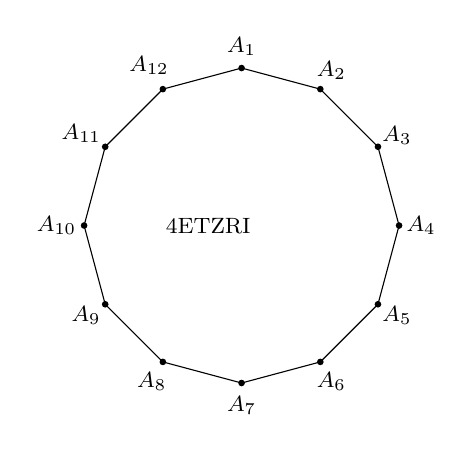
\begin{tikzpicture}[scale=1, font=\footnotesize, line join=round, line cap=round, >=stealth]
    %hidden: VM005
			\foreach \i in {1,...,12}{
			\pgfmathsetmacro{\ang}{90-(\i-1)*30}
			\coordinate (A\i) at (\ang:2);
			}
			\draw (A1) \foreach \i in {2,...,12}{--(A\i)} -- cycle;
			\foreach \i in {1,...,9}{
			\pgfmathsetmacro{\ang}{90-(\i-1)*30}
			\fill (A\i) circle(1.2pt);
			\node[shift={(\ang:0.28)}] at (A\i) {$A_{\i}$};
			}
			\foreach \i in {10,11,12}{
			\pgfmathsetmacro{\ang}{90-(\i-1)*30}
			\fill (A\i) circle(1.2pt);
			\node[shift={(\ang:0.35)}] at (A\i) {$A_{\i}$};
			}
    \node at (0,0){\href{4ETZRI}{\tiny \phantom{4ETZRI}}};
		\end{tikzpicture}	
		}
		\par \shortans{$1\,856$}
	\loigiai{
		Vì các bóng đèn có công suất đôi một khác nhau nên tổng số cách lắp $12$ bóng đèn vào $12$ đỉnh là $12!$. 
		Tuy nhiên, biến cố đang xét chỉ phụ thuộc vào vị trí của $4$ bóng màu đỏ. Mỗi cách chọn $4$ vị trí cho bóng đỏ ứng với $4!\cdot 8!$ cách lắp các bóng cụ thể, do đó ta chỉ cần xét cách chọn $4$ đỉnh đặt bóng đỏ trong $12$ đỉnh.\\
		Tổng số cách chọn vị trí cho $4$ bóng đỏ là $\mathrm{C}_{12}^4=495$.\\
		Trong đa giác đều $12$ cạnh, các hình vuông có bốn đỉnh là đỉnh của đa giác là
		$A_1A_4A_7A_{10}$, $A_2A_5A_8A_{11}$, $A_3A_6A_9A_{12}$.\\
		Ba hình vuông này chia $12$ đỉnh của đa giác thành $3$ nhóm, mỗi nhóm có $4$ đỉnh.\\
		Để mỗi hình vuông đều có ít nhất một bóng đỏ, vì có $4$ bóng đỏ và $3$ hình vuông nên số bóng đỏ trên ba hình vuông phải được phân bố $2-1-1$.\\
		Số cách chọn vị trí thỏa mãn là
		$3 \cdot \mathrm{C}_4^2\cdot \mathrm{C}_4^1\cdot \mathrm{C}_4^1
		=3\cdot 6\cdot 4\cdot 4=288$.\\
		Suy ra $P=\dfrac{288}{495}=\dfrac{32}{55}$.\\
		Vậy $3\,190P=3\,190\cdot \dfrac{32}{55}=1\,856$.
	}
\end{ex}

\begin{ex}%[Dự án 2BT3BO-VN-MT-15+]%[2-TN-0103-BGD-2026,VM021]%[0C1V1-3]
	Một nông trại cung cấp rau quả cho siêu thị A với số liệu bán hàng của bốn ngày trong tuần được ghi lại trong bảng sau:
	\begin{center}
		\renewcommand{\arraystretch}{1.3}
		\begin{tabular}{|c|c|c|c|c|}
			\hline
			\multirow{2}{*}{Ngày} & \multicolumn{3}{c|}{Số ki-lô-gam} & \multirow{2}{*}{\makecell{Tổng số tiền \\ (nghìn đồng)}} \\
			\cline{2-4}
			& Rau muống & Bí xanh & Cà chua & \\
			\hline
			Thứ Tư & $19$ & $14$ & $10$ & $600$ \\
			\hline
			Thứ Năm & $20$ & $12$ & $8$ & $540$ \\
			\hline
			Thứ Sáu & $25$ & $12$ & $7$ & $570$ \\
			\hline
			Thứ Bảy & $50$ & $25$ & $20$ & $?$ \\
			\hline
		\end{tabular}
	\end{center}
	Biết rằng đơn giá theo ki-lô-gam của mỗi loại rau quả trong bảng trên là không đổi. Tổng số tiền nông trại thu được ở ngày thứ Bảy từ ba loại rau quả trên khi cung cấp cho siêu thị A là bao nhiêu nghìn đồng?
	\par \shortans{$1\,275$}
	\loigiai{
		Gọi $x$, $y$, $z$ (nghìn đồng) lần lượt là đơn giá của $1$ ki-lô-gam rau muống, bí xanh và cà chua.\\
		Từ số liệu của ba ngày Thứ Tư, Thứ Năm, Thứ Sáu, ta có hệ phương trình
		\[\heva{&19x+14y+10z=600\\&20x+12y+8z=540\\&25x+12y+7z=570} 
		\Leftrightarrow \heva{& x=10\\ &y=15 \\ &z=20.}\]
		Suy ra tổng số tiền thu được trong ngày Thứ Bảy là
		\[50x+25y+20z=50\cdot 10+25\cdot 15+20\cdot 20=1\,275\ (\text{nghìn đồng}).\]
		Vậy tổng số tiền nông trại thu được trong ngày Thứ Bảy là $1\,275$ nghìn đồng.
	}
\end{ex}

\begin{ex}%[Dự án ZDBRKQ-VN-MT-15+]%[2-TN-0103-BGD-2026,TV015]%[2D4V3-5]
	Để chế tác một hạt cườm, người ta lấy một khối vật thể có dạng một khối tròn xoay được tạo thành khi quay hình phẳng giới hạn bởi trục $Ox$ và nửa trên của elip $\dfrac{x^2}{1{,}5^2} + \dfrac{y^2}{1^2} = 1$ (một đơn vị dài trên mỗi trục tọa độ tương ứng với một xăng-ti-mét trong thực tế) quanh trục $Ox$; sau đó khoan dọc theo trục xoay như hình vẽ sau:
	\begin{center}
		\begin{tikzpicture}[scale=1.4, font=\footnotesize, line join=round, line cap=round, >=stealth]
    %hidden: VM005
			\tikzset{declare function={R=1.5;r=0.2;Rb=1;r1=0.87;goc=asin(r/Rb);x0=R*cos(goc);}}
			%Mũi khoan
			\fill[gray] (-Rb,-r)--(-Rb,r)--(2*r,r)--(2.5*r,0)--(2*r,-r)--cycle;
			\path (-2*r,0)node[shift=(90:0.5)]{Mũi khoan};
			% Hình 2D bên trái
			\begin{scope}[xshift=2.2cm]
				\draw[dashed] (0,-Rb)--(0,Rb) (-R,0)--(R,0)(-x0,-r) --++ (2*x0,0) (-x0,r) --++ (2*x0,0) (0,Rb) arc (90:-90:{Rb/4} and {Rb}) (-R/2,r1) arc (90:-90:{r1/4} and {r1}) (R/2,r1) arc (90:-90:{r1/4} and {r1});
				\draw (0,0) node[shift=(-135:6pt)] {$O$} (0,0) ellipse ({R} and {Rb}) (-1.12*R,0)--(-R,0) (0,-1.3*Rb)--(0,-Rb) (0,Rb) arc (90:270:{Rb/4} and {Rb}) (-R/2,r1) arc (90:270:{r1/4} and {r1}) (R/2,r1) arc (90:270:{r1/4} and {r1});
				\draw[->] (R,0) -- (1.2*R,0) node[below] {$x$};
				\draw[->] (0,Rb) -- (0,1.5*Rb) node[left] {$y$};
				\draw[<-] (-R-0.05,0)--++(225:Rb)node[shift=(-90:0.2)]{Trục xoay};
				\draw[<->](-R+r,0)--++(0,r);
				\draw[<-] (-R+r,r)--++(135:Rb)node[shift=(90:0.2)]{Bán kính lỗ khoan $0{,}2$};
				\path (R/2,r1)node[shift=(90:0.5)]{$\tfrac{x^2}{1{,}5^2}+\tfrac{y^2}{1^2}=1$};
			\end{scope}
			% Hình 3D ở giữa
			\begin{scope}[xshift=5.8cm]
				\fill[brown!70] (x0, r) arc (goc:180-goc:{R} and {Rb}) -- (-x0, r) -- cycle;
				\fill[brown!70] (x0, -r) arc (-goc:-180+goc:{R} and {Rb}) -- (-x0, -r) -- cycle;
				\draw[dashed] (-x0,-r) --++ (2*x0,0) (-x0,r) --++ (2*x0,0) (0,Rb) arc (90:-90:{Rb/4} and {Rb}) ;
				\draw  (0,0) ellipse ({R} and {Rb}) (0,Rb) arc (90:270:{Rb/4} and {Rb}) ;
				\draw[fill=white] (x0, 0) ellipse ({r/6} and r);
				\fill[white] (-x0, 0) ellipse ({r/4} and r);
				\draw[dashed](-x0,r) arc (90:-90:{r/6} and {r});
				\draw (-x0,r) arc (90:270:{r/6} and {r});
			\end{scope}
			%Hình mặt cắt bên phải
			\begin{scope}[xshift=9.2cm]
				\fill[pattern=north west lines,opacity=.7] (x0, r) arc (goc:180-goc:{R} and {Rb})--cycle;
				\path (R/2,r1)node[shift=(90:0.5)]{$\tfrac{x^2}{1{,}5^2}+\tfrac{y^2}{1^2}=1$};
				\draw[->] (-R-r,0) -- (1.3*R,0) node[below] {$x$};
				\draw[->] (0,-0.35) -- (0,1.5*Rb) node[left] {$y$};
				\draw (-R-r,r) -- (1.3*R,r) node[shift=(90:0.2)]{$y=0{,}2$}
					(x0, r) arc (goc:180-goc:{R} and {Rb});
				\fill (0,0) node{\href{ZDBRKQ}{\tiny \phantom{ZDBRKQ}}} circle(0.5pt) node[shift=(-135:0.25)]{$O$}; 
			\end{scope}
    \node at (0,0){\href{ZDBRKQ}{\tiny \phantom{ZDBRKQ}}};
		\end{tikzpicture}
		\textit{Lưu ý: Các kích thước trong hình minh họa có thể không đúng tỉ lệ thực tế.}
	\end{center}
	Lỗ khoan có dạng hình trụ với bán kính $0{,}2$\,cm và có trục nằm trên trục xoay. Phần còn lại sau khi khoan là hạt cườm, có dạng một khối tròn xoay. Thể tích của hạt cườm đó bằng bao nhiêu xăng-ti-mét khối {\it(không làm tròn kết quả các phép tính trung gian, chỉ làm tròn kết quả cuối cùng đến hàng phần trăm)}?
	\par\shortans{$5{,}91$}
	\loigiai{
		Nửa trên của elip có phương trình là $y = \sqrt{1 - \dfrac{x^2}{1{,}5^2}} = \sqrt{1 - \dfrac{x^2}{2{,}25}}$ với $x \in [-1,5; 1,5]$.\\
		Lỗ khoan có dạng hình trụ bán kính $r = 0{,}2$\,cm dọc theo trục xoay $Ox$.\\
		Khi đó, giới hạn của hạt cườm theo trục $Ox$ là phần nằm giữa hai giao điểm của nửa elip với đường thẳng $y = 0{,}2$.\\
		Phương trình hoành độ giao điểm của $y=\sqrt{1 - \dfrac{x^2}{2{,}25}}$ và $y= 0{,}2$ là
		\allowdisplaybreaks
		\begin{eqnarray*}
			\sqrt{1 - \dfrac{x^2}{2{,}25}} = 0{,}2 &\Leftrightarrow &1 - \dfrac{x^2}{2{,}25} = 0{,}04 \\
			&\Leftrightarrow &x^2 = 2{,}16\\
			&\Leftrightarrow &\hoac{&x_1=-\sqrt{2{,}16}\\&x_2=\sqrt{2{,}16}.}
		\end{eqnarray*}
		Khi đó, phần vật thể hạt cườm là khối tròn xoay được giới hạn bởi các mặt phẳng $x = x_1$, $x = x_2$ và có thiết diện tại mỗi hoành độ $x$ là một hình vành khăn với bán kính ngoài là $y(x)$ và bán kính trong là $r = 0{,}2$.\\
		Thể tích của hạt cườm là
		\allowdisplaybreaks
		\begin{align*}
			V &=\pi \displaystyle\int\limits_{x_1}^{x_2} \left(1 - \dfrac{x^2}{2{{,}}25} - 0{,}04\right) \mathrm{d}x\\
			&=2\pi \displaystyle\int\limits_{0}^{x_2} \left(\dfrac{24}{25} - \dfrac{4}{9}x^2\right) \mathrm{d}x\\
			&=2\pi\left(\dfrac{24}{25}x - \dfrac{4}{27}x^3\right)\Bigg|_0^{x_2}\approx 5{,}91.
		\end{align*}
		Vậy thể tích của hạt cườm gần bằng $5{,}91$\,cm$^3$.
	}
\end{ex}

\begin{ex}%[Dự án 49WX93-VN-MT-15+]%[2-TN-0103-BGD-2026,TV015]%[0D8C2-3]
	Trong một trò chơi bạn Bình cần vượt qua một thử thách. Theo yêu cầu của thử thách, Bình cần điền tất cả $15$ số thuộc tập hợp $\{0; 1; 2; 3; 4; 5; 6; 7; 8; 10; 11; 12; 15; 16; 20\}$ vào $15$ ô vuông trong hình dưới thỏa mãn đồng thời ba điều kiện sau:
	\begin{itemize}
		\item Mỗi ô điền đúng một số và mỗi số chỉ được sử dụng một lần;
		\item Hiệu hai số ở hai ô bất kì khác nhau trên cùng một hàng không chia hết cho $5$;
		\item Hiệu hai số ở hai ô bất kì khác nhau trên cùng một cột không chia hết cho $5$.
	\end{itemize}
	Hai cách điền gọi là giống nhau nếu số điền ở mỗi ô tương ứng trong $15$ ô là giống nhau (không tính đến thứ tự điền các số vào $15$ ô vuông). Gọi $H$ là số cách điền khác nhau để bạn Bình vượt qua được thử thách. Giá trị của $\dfrac{H}{30}$ bằng bao nhiêu?
	\begin{center}
		\begin{tikzpicture}[scale=1.2, font=\footnotesize, line join=round, line cap=round, >=stealth]
    %hidden: VM005
			\foreach \i in {1,...,5} {
			\foreach \j in {1,...,\i} {
			\draw (\j-1, 5-\i) rectangle (\j, 6-\i);
			}
			}
			\node[left] at (0, 0.5) {Hàng 1};
			\node[left] at (0, 1.5) {Hàng 2};
			\node[left] at (0, 2.5) {Hàng 3};
			\node[left] at (0, 3.5) {Hàng 4};
			\node[left] at (0, 4.5) {Hàng 5};
			\node[below] at (0.5, 0) {Cột 1};
			\node[below] at (1.5, 0) {Cột 2};
			\node[below] at (2.5, 0) {Cột 3};
			\node[below] at (3.5, 0) {Cột 4};
			\node[below] at (4.5, 0) {Cột 5};
    \node at (0,0){\href{49WX93}{\tiny \phantom{49WX93}}};
		\end{tikzpicture}
	\end{center}
	\par\shortans{$1\,152$}
	\loigiai{
		Chia tập hợp đã cho thành các nhóm theo số dư khi chia cho $5$:\\
		$S_0 = \big\{0; 5; 10; 15; 20\big\}$, $S_1 = \big\{1; 6; 11; 16\big\}$, $S_2 = \big\{2; 7; 12\big\}$, $S_3 = \big\{3; 8\big\}$, $S_4 = \big\{4\big\}$.\\
		Gọi $A_i$ là tập các ô chứa các phần tử thuộc $S_i$ với $i\in \big\{1;2;3;4\big\}$.\\
		Do hiệu hai số trên cùng hàng hoặc cùng cột không chia hết cho $5$ nên các ô thuộc cùng một $A_i$ không được nằm trên cùng hàng hoặc cùng cột.\\
		Xét $A_0$ gồm $5$ ô.\\
		Vì bảng có $5$ hàng và $5$ cột nên mỗi hàng và mỗi cột chứa đúng một ô thuộc $A_0$.\\
		Suy ra các vị trí của $A_0$ được xác định duy nhất trên đường chéo phụ là
		\[A_0 = \big\{(1;5), (2;4), (3;3), (4;2), (5;1)\big\}.\]
		Lập luận tương tự, ta cũng có\\
		$A_1 = \big\{(1;4), (2;3), (3;2), (4;1)\big\}$, $A_2 = \big\{(1;3), (2;2), (3;1)\big\}$, $A_3 = \big\{(1;2), (2;1)\big\}$, $A_4 = \big\{(1;1)\big\}$.\\
		Số cách xếp các phần tử lần lượt là $A_0$ có $5!$ cách, $A_1$ có $4!$ cách, $A_2$ có $3!$ cách, $A_3$ có $2!$ cách và $A_4$: $1!$ cách.\\
		Suy ra $H = 5! \cdot 4! \cdot 3! \cdot 2! \cdot 1! = 34\,560$.\\
		Vậy $\dfrac{H}{30} = \dfrac{34\,560}{30} = 1\,152$.
	}
\end{ex}

\begin{ex}%[Dự án 3OSDOY-VN-MT-15+]%[2-TN-0103-BGD-2026,TV013]%[2D1V3-6]
	Một công ty nông sản có công suất chế biến không quá $200$ tấn nguyên liệu một tháng. Nếu công ty chế biến $x$ tấn nguyên liệu trong một tháng ($1 \leq x \leq 200$) thì chi phí sản xuất và doanh thu lần lượt là $C(x)=0{,}001x^3+30x+10$ (triệu đồng) và $R(x)=60x$ (triệu đồng). Lợi nhuận lớn nhất mà công ty đạt được trong một tháng là bao nhiêu triệu đồng?
	\par \shortans{$1\,990$}
	\loigiai{
		Với $x \in [1; 200]$ thì hàm số biểu thị lợi nhuận của công ty trong một tháng là
		\[P(x) = R(x) - C(x) = 60x - \left(0{,}001x^3 + 30x + 10\right) = -0{,}001x^3 + 30x - 10.\]
		Ta có $P'(x) = -0{,}003x^2 + 30$.\\
		Phương trình $P'(x) = 0 \Leftrightarrow -0{,}003x^2 + 30 = 0 \Leftrightarrow x^2 = 10\,000 \Rightarrow \hoac{&x = 100 \in [1; 200] \\ &x = -100 \notin [1; 200].}$\\
		Bảng biến thiên của hàm số $P(x)$ trên đoạn $[1; 200]$ là
		\begin{center}
			\begin{tikzpicture}
    %hidden: VM005
				\tkzTabInit[nocadre=true, lgt=1.3, espcl=4, deltacl=0.7]
				{$x$/0.7, $P'(x)$/0.7, $P(x)$/2.5}
				{$1$, $100$, $200$}
				\tkzTabLine{,+,$0$,-,}
				\tkzTabVar{-/$19{,}999$, +/$1\,990$, -/$-2\,010$} 
    \node at (T11){\href{3OSDOY}{\tiny \phantom{3OSDOY}}};
			\end{tikzpicture}
		\end{center}
		Từ bảng biến thiên, ta thấy $\max\limits_{[1; 200]} P(x) = P(100) = 1\,990$.\\
		Vậy lợi nhuận lớn nhất mà công ty đạt được trong một tháng là $1\,990$ triệu đồng.
	}
\end{ex}

\begin{ex}%[Dự án 117TZ8-VN-MT-15+]%[2-TN-0103-BGD-2026,TV013]%[2H5V1-5]
	Cho hình lập phương $ABCD.MNPQ$ có cạnh bằng $6$. Gọi $E$ là trung điểm của đoạn thẳng $AB$. Khoảng cách từ điểm $P$ đến mặt phẳng $(MED)$ bằng bao nhiêu (\textit{không làm tròn kết quả các phép tính trung gian, chỉ làm tròn kết quả cuối cùng đến hàng phần trăm})?
	\par \shortans{$7{,}35$}
	\loigiai{
		\textit{\underline{Cách 1}: Phương pháp tọa độ hóa.}
		\begin{center}
			\begin{tikzpicture}[declare function={r=4;}, font=\footnotesize, line join=round, line cap=round, >=stealth]
    %hidden: VM005
				\path
					(0:0) coordinate (A)
					(0:r) coordinate (B)
					++(37:{0.65*r}) coordinate (C)
					++(180:r) coordinate (D)
					\foreach \x in {A,B,C,D}{(\x)++(90:r) coordinate (\x_1)};
				\coordinate (M) at (A_1);
				\coordinate (N) at (B_1);
				\coordinate (P) at (C_1);
				\coordinate (Q) at (D_1);
				\coordinate (E) at ($(A)!0.5!(B)$);
				\draw[->] (B) -- ($(A)!1.3!(B)$) node[below] {$x$};
				\draw[->] (D) -- ($(A)!1.4!(D)$) node[above] {$y$};
				\draw[->] (M) -- ($(A)!1.3!(M)$) node[left] {$z$};
				\draw[dashed] (Q)--(D)--(A) (D)--(C) (M)--(D) (E)--(D);
				\draw (A)--(B)--(C) (A)--(M) (B)--(N) (C)--(P) (M)--(N)--(P)--(Q)--cycle (M)--(E);
				\foreach \x/\goc/\t in {A/225/O\equiv A, B/-90/B, C/0/C, D/180/D, M/135/M, N/-45/N, P/45/P, Q/135/Q, E/-90/E}{
				\fill (\x) circle (1pt) node[shift={(\goc:9pt)}]{$\t$};
			}
    \node at (0,0){\href{117TZ8}{\tiny \phantom{117TZ8}}};
			\end{tikzpicture}
		\end{center}
		Chọn hệ trục tọa độ $Oxyz$ sao cho gốc tọa độ $O$ trùng với đỉnh $A$, các tia $Ox$, $Oy$, $Oz$ lần lượt chứa các cạnh $AB$, $AD$, $AM$ như hình vẽ.\\
		Vì hình lập phương có cạnh bằng $6$ nên ta có tọa độ các đỉnh là
		$A(0;0;0)$, $B(6;0;0)$, $D(0;6;0)$, $M(0;0;6)$.\\
		Đỉnh $C$ thuộc mặt phẳng $(Oxy)$ sao cho $ABCD$ là hình vuông nên $C(6;6;0)$.\\
		Đỉnh $P$ nằm trên $C$ một đoạn $6$ đơn vị (cùng phía với tia $Oz$) nên $P(6;6;6)$.\\
		Vì $E$ là trung điểm của $AB$ nên $E(3;0;0)$.\\
		Mặt phẳng $(MED)$ đi qua ba điểm $M(0;0;6)$, $E(3;0;0)$, $D(0;6;0)$.\\
		Áp dụng phương trình mặt phẳng theo đoạn chắn, ta có phương trình mặt phẳng $(MED)$ là
		\[\dfrac{x}{3} + \dfrac{y}{6} + \dfrac{z}{6} = 1 \Leftrightarrow 2x + y + z - 6 = 0.\]
		Khoảng cách từ điểm $P(6;6;6)$ đến mặt phẳng $(MED)$ là
		\[\mathrm{d}\big(P, (MED)\big) = \dfrac{|2 \cdot 6 + 6 + 6 - 6|}{\sqrt{2^2 + 1^2 + 1^2}} = \dfrac{18}{\sqrt{6}} = 3\sqrt{6} \approx 7{,}35.\]		
		\textit{\underline{Cách 2}: Phương pháp hình học thuần túy.}
		\begin{center}
			\begin{tikzpicture}[declare function={r=4;}, font=\footnotesize, line join=round, line cap=round, >=stealth]
    %hidden: VM005
				\path (0:0) coordinate (A)
					(0:r) coordinate (B)
					++(37:{0.65*r}) coordinate (C)
					++(180:r) coordinate (D)
					\foreach \x in {A,B,C,D}{(\x)++(90:r) coordinate (\x_1)};
				\coordinate (M) at (A_1);
				\coordinate (N) at (B_1);
				\coordinate (P) at (C_1);
				\coordinate (Q) at (D_1);
				\coordinate (E) at ($(A)!0.5!(B)$);
				\coordinate (K) at (intersection of A--C and E--D);
				\coordinate (I) at (intersection of A--P and M--K);
				\draw[dashed] (Q)--(D)--(A) (D)--(C) (M)--(D) (E)--(D) (A)--(C) (A)--(P) (C)--(M)--(K);
				\draw (A)--(B)--(C) (A)--(M) (B)--(N) (C)--(P) (M)--(N)--(P)--(Q)--cycle (M)--(E) (M)--(P);
				\foreach \x/\goc/\t in {A/225/A, B/-90/B, C/0/C, D/30/D, M/135/M, N/90/N, P/45/P, Q/135/Q, E/-90/E, K/-30/K, I/90/I}{
				\fill (\x) circle (1pt) node[shift={(\goc:9pt)}]{$\t$};
			}
    \node at (0,0){\href{117TZ8}{\tiny \phantom{117TZ8}}};
			\end{tikzpicture}
		\end{center}
		Tứ diện $A.MED$ có $AM \perp (ABCD)$ nên $AM \perp AD$ và $AM \perp AE$, đồng thời $ABCD$ là hình vuông nên $AE \perp AD$.\\
		Do đó $A.MED$ là tứ diện vuông tại đỉnh $A$.\\
		Gọi $h$ là khoảng cách từ $A$ đến mặt phẳng $(MED)$. Ta có
		\[\dfrac{1}{h^2} = \dfrac{1}{AM^2} + \dfrac{1}{AE^2} + \dfrac{1}{AD^2} = \dfrac{1}{6^2} + \dfrac{1}{3^2} + \dfrac{1}{6^2} = \dfrac{6}{36} = \dfrac{1}{6} \Rightarrow h = \sqrt{6}.\]
		Trong mặt phẳng $(ABCD)$, gọi $K = AC \cap ED$.\\
		Vì $AE \parallel CD$ nên $\triangle AKE \backsim \triangle CKD$.\\
		Suy ra $\dfrac{AK}{KC} = \dfrac{AE}{CD} = \dfrac{1}{2} \Rightarrow AK = \dfrac{1}{3}AC$.\\
		Trong mặt phẳng $(MAC)$, gọi $I = AP \cap MK$.\\
		Vì $MK \subset (MED)$ nên $I$ chính là giao điểm của $AP$ và mặt phẳng $(MED)$.\\
		Tứ giác $AMCP$ là hình chữ nhật nên $AK \parallel MP$.\\
		Áp dụng định lý Thalès trong tam giác $\triangle PIM$, ta có
		\[\dfrac{IA}{IP} = \dfrac{AK}{MP} = \dfrac{\dfrac{1}{3}AC}{AC} = \dfrac{1}{3}.\]
		Do $A$, $I$, $P$ thẳng hàng và $I$ nằm giữa $A$ và $P$ nên ta thiết lập được tỉ số khoảng cách
		\[\dfrac{\mathrm{d}\big(P, (MED)\big)}{\mathrm{d}\big(A, (MED)\big)} = \dfrac{IP}{IA} = 3 \Rightarrow \mathrm{d}\big(P, (MED)\big) = 3 \cdot \mathrm{d}\big(A, (MED)\big) = 3\sqrt{6} \approx 7{,}35.\]
		Vậy khoảng cách từ điểm $P$ đến mặt phẳng $(MED)$ bằng $7{,}35$.
	}
\end{ex}

\Closesolutionfile{ans}
\Closesolutionfile{ansbook}
\begin{indapan}
	{ans/ans\currfilebase}
\end{indapan}